\documentclass[review]{elsarticle}

\usepackage{lineno,hyperref}
\usepackage{amsmath,amsfonts,amsthm,amssymb} % nice math symbols
\usepackage{graphicx}
\graphicspath{{../../images/}}

\usepackage[plain]{algorithm}
\usepackage[noend]{algpseudocode}
\renewcommand{\algorithmiccomment}[1]{{\quad\footnotesize // #1}}
\renewcommand{\algorithmicrequire}{\textbf{Input:}}
\renewcommand{\algorithmicensure}{\textbf{Output:}}

\newtheorem{definition}{Defenition}

\modulolinenumbers[5]

\journal{Knowledge-Based Systems}

%%%%%%%%%%%%%%%%%%%%%%%
%% Elsevier bibliography styles
%%%%%%%%%%%%%%%%%%%%%%%
%% To change the style, put a % in front of the second line of the current style and
%% remove the % from the second line of the style you would like to use.
%%%%%%%%%%%%%%%%%%%%%%%


%% `Elsevier LaTeX' style
\bibliographystyle{elsarticle-num}
%%%%%%%%%%%%%%%%%%%%%%%

\begin{document}

\begin{frontmatter}

\title{Relationships and operations in agent's sign-based model of the world}

%% or include affiliations in footnotes:
\author{Gennady S. Osipov\corref{mycorrespondingauthor}}
\ead{gos@isa.ru}

\author{Aleksandr I. Panov\corref{mycorrespondingauthor}}
\ead{pan@isa.ru}

\cortext[mycorrespondingauthor]{Corresponding author}

\address{Federal Research Center ``Computer Science and Control'' Russian Academy of Sciences, Moscow, Russia}

\begin{abstract}
According to modern theories of mental function's emergence and the role of neurophysiological processes therein, the mental function formation is associated with the existence or communicative synthesis of specific information structures containing three information types of different origin: information coming from the external environment, information extracted from the memory and information coming from motivation centres. The binding of these components into a single entity is ensured by naming them; this also provides for the emerging structures’ stability. We call such information structures as signs due to their resemblance to similar structures that have been studied in semiotics. The set of signs formed by the actor during activities and communication forms his sign based world model reflecting his ideas about the environment, himself and other actors.

The sign based world model enables the setting and resolution of a number of tasks arising for intelligent agents and their coalitions during behaviour modeling , such as goal-setting, purposeful behaviour synthesis, role distribution, and the interaction of agents in the coalition. The paper considers a special object - the causal matrix, which describes the structure of the sign components. Operations and relationships in the sign based world model simulating of the psychological characteristics of human behaviour are determined on this basis.
\end{abstract}

\begin{keyword}
sign based world model \sep sign image \sep sign significance \sep sign personal meaning \sep causal matrix \sep semiotic network \sep script generation \sep agglutination \sep generalization
\end{keyword}

\end{frontmatter}

\linenumbers

\section*{Introduction}
Apparently, the issue of feeling occurrence is one of the central issues of cognitive psychology. Also, there is no clarity regarding the relationship of this phenomenon to the actor’s world model formation. In psychologists’ works, such as those by A. N. Leontiev \cite{Leontiev2009,Igira2009}, the representation of each object or reality phenomenon in the mind consists of three components: an image of the object, its cultural and historical meaning, and personal meaning. According to the image concept developed in cognitive psychology, perception is considered to be a categorization process, and the meaning corresponds to the object’s mission, the sign’s semantic component, and the personal meaning is interpreted as a set of actions regarding the object as preferred by the actor. It is easy to notice that this structure is close to the structure named as a sign in semiotics \cite{Pierce2000b,Frege2000}, so the approach developed in this paper can be pertinently called a sign-oriented or semiotic approach. The structure of the world model described above is supported not only by the cultural and historical approach, but by other psychological theories as well, particularly by Stanovich’s three-process model \cite{Stanovich2009}. According to this, unlike the well-known two-process model by Kahneman \cite{Kahneman2011}, mental processes are implemented by three subsystems: reflective, algorithmic and autonomous ones.

These considerations are supported by the results of many neurosurgery studies, first of all \cite{Ivanitsky1996}, which associate feeling occurrence, i.e. the transition from the neurophysiological level to the psychological level, with the circular motion of the excitation of part of the brain cortex, which returns to the place of the original signal projection after further processing by other brain structures (the ``feeling circle''). The mental function \cite{Ivanitsky2010} is based on the synthesis of three information types (i.e. forming ternary structures): information coming from the external environment (sensory information), and information extracted from the memory and information coming from motivation centres. We should note that the works \cite{Edelmen1981} also indicate the possibility of the presence of the sign structure in the activity actors’ world model, and \cite{Friederici2015} considers the mechanism for forming some cognitive functions and its relationship with the formation of the linguistic world model. The work \cite{Loula2012} deals with the emergence of communication mechanisms based on a semiotic approach. In \cite{Roy2005}, Roy suggested the sign based model of the world as the basis of robots’ operating component.

In subsequent years, the application of the idea of returning excitation to explain the mechanisms of consciousness and the ``sign'' hypothesis has been supported by the results of many studies, including data gathered on the structure of those brain parts involved in the ``feeling circle''. The sign components are neurally realized in various subsystems of the brain. The image component of the sign is realized through the distribution of neural activation from the primary sensory sections of the cortico-thalamic system to the associative ones. The researchers describe two ways for such activation to take place: the lower (ventral) stream determines spatially independent object characteristics of the incoming sensory information and the back (dorsal) stream recognizes the spatial configuration and actions \cite{Grossberg2014}. The existence of these two activation flows justifies the existence of object and procedural features in the sign's image component (section \ref{sec:structure}).

The existence of the process of image recognition, in which predicting feedback of the neurons’ preactivation (details in section \ref{subsec:actual}) places a role, creates the effect of re-entering into the primary cortex sections \cite{Edelmen1981,Ivanitsky1996}. The personal meaning component is a product of interaction between the cortex motor sections and subcortical structures, such as thalamus, basal ganglia, amygdala and hypothalamus. These brain subsystems implement the integration of the previous action experience and the action choice in the current situation, taking into account the current motive and purpose \cite{Gurney2001}. The hippocampus is also closely related to the personal meaning component, and it plays an important role in the episodic memory formation, i.e. a description of the current and recent activity situation \cite{Rolls2010}. Finally, the meaning component is the result of the generalizing and abstracting brain function, which is realized by the frontal and superior temporal sections of the brain cortex. These sections are also involved in the binding of all sign components with their subsequent naming \cite{Friederici2015,Pulvermuller2013}.

In section \ref{sec:sintaxis}, we will describe a high-level conceptual part of the model; we will not delve into sign structure details but instead describe the general scheme of its formation and its syntax determination. Section \ref{sec:semantic} provides an interpretation of the sign components through the use of a predicate logic and rule system (operational semantics). Further, the main attention will be paid to the neurophysiologically and psychologically plausible sign based model and its structure (section \ref{sec:structure}). At the structural level, basic mathematical objects will be suggested, sign components determined, and the algorithm of the image component described. Further, a structural definition is given to the basic relationship groups of the sign components and the concept of semiotic network as the world model simulation is introduced (section \ref{sec:semnetwork}). To demonstrate the constructed model’s applicability, section \ref{sec:operations} covers basic operations in the world model, simulating the known cognitive functions: generalization, script formation and the meaning agglutination.

\section{Syntactic level}\label{sec:sintaxis}

We determine the syntactic level of the world model simulation according to the works \cite{Osipov2014c,Osipov2015c}. Let there be given a set $S$ called the sign set. Each element $s\in S$ has the form $s=\langle n,p,m,a\rangle$, where $n\in N$, $p\subseteq P$, $a\subseteq A$, $m\subseteq M$. Here, $N$ --- is a set of finite length words in some alphabet, which we call the name set; $P$ --- is a set of closed atomic formulas of the first order predicate calculus, which we call the property set; $M$ --- will be called the significance set; and $A$ --- is the meaning set. Both the significance set $M$ and the meaning set $A$ are interpreted by a set of actions due to psychological considerations. As done regarding Artificial Intelligence, we represent every action through the rule \cite{Osipov2002b}. The rule is an ordered triple of sets $r=\langle Con,Add,Del\rangle$, where $Con$ --- is the rule condition; $Add$ --- is a set of facts added by the rule $r$; and $Del$ --- is a set of facts deleted by the rule $r$. In a general case, each of these sets is a set of atomic formulas of the first order predicate calculus. In more detail, the role of these rules in the sign based model will be described in the next section.

Now, let us introduce linking operators. $\Psi_p^m:2^P\rightarrow 2^M$ --- is the operator coupling the image $p$ with the significance $m$. The second operator $\Psi_m^a:2^M\rightarrow 2^A$ associates the significances with the meanings. The third operator $\Psi_a^p: 2^A\rightarrow 2^P$ associates the meanings with the images. The operators that are introduced associate the sign components with one another, and their semantics are determined in the next section. At the syntactic level of the  model, the basic algorithms are determined: the sign formation and self-organizing procedures \cite{Osipov2014c}.

\section{Semantic level of the model}\label{sec:semantic}

At the semantic level of the world model simulation, the operational semantics of the linking operators introduced at the syntactic level are specified, and the sign components are interpreted by the set of predicate calculus symbols and the rules determined in the artificial intelligence \cite{Osipov2015c,Osipov2016a}.

Let us determine the linking operator (Figure \ref{fig:linkers}) $\Psi_p^m(p^{(i)})=m^{(i)}$, so that $m^{(i)}=\{r|\mathcal{P}_c(r)\subseteq \mathcal{P}(p^{(i)})\}$, where $\mathcal{P}_c(r)$ is a set of different predicate symbols of the condition rule $r$ interpreting the significance $m$ (hereinafter, we will associate one action, i.e. one rule, with each significance for the explanation simplicity); $\mathcal{P}(p^{(i)})$ --- is the set of image predicate symbols $p^{(i)}$; $p^{(i)}\in 2^P$, $m^{(i)}\in 2^M$, $2^P$ and $2^M$ are $P$ and $M$ Booleans respectively.


\begin{figure}[H]
	\label{fig:linkers}
	\centering
	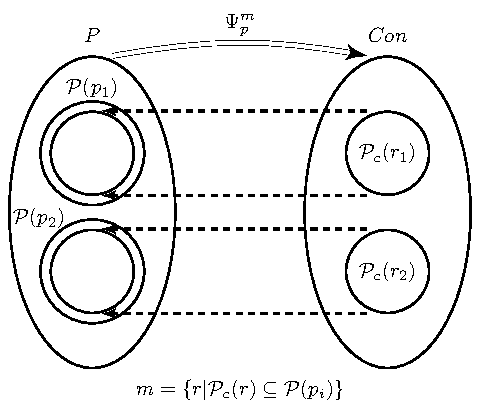
\includegraphics[width=0.32\textwidth,page=1]{sign-schemas/oper_relat}
	\includegraphics[width=0.32\textwidth,page=2]{sign-schemas/oper_relat}
	\includegraphics[width=0.32\textwidth,page=3]{sign-schemas/oper_relat}
	\caption{Schemes of linking operators.}		
\end{figure}

The second operator $\Psi_m^a(m^{(i)})=a^{(i)}$, where  $a^{(i)}=\{r^*|\mathcal{P}_c(r)\cap \mathcal{P}_c(r^*)\not=\varnothing\}$, where $\mathcal{P}_c(r)$ --- is the set of rule $r^*$ condition predicate symbols $Con$ interpreting the personal meaning $a^{(i)}$ (here, same as in the significance case, each personal meaning is associated with one action, i.e. one rule, for the explanation simplicity); $m^{(i)}\in 2^M, a^{(i)}\in 2^A$, $2^A$ --- is Boolean $A$. The third operator $\Psi_a^p(a^{(i)})=p^{(i+1)}$, where $p^{(i+1)}\subseteq \mathcal{P}_a(r_j^*)$, $a^{(i)}\in 2^A$, $p^{(i+1)}\in 2^P$,, where $\mathcal{P}_a(r_j^*)$ is the set of predicate symbols from addition set of the rule $r_j^*$ .

Of course, $p^{(i)}\not = p^{(i+1)}$. It can be shown that under certain initial approximation, this iterative process converges to $p$, wherein, $\|\mathcal P_c(r)\cap\mathcal P_c(r^*)\|\geq 2$. It is easy to see that a sufficient convergence condition is $\mathcal P_c(r)\subseteq\mathcal P_c(r^*)$. If we introduce operator $\Psi_m^p=\Psi_a^p\Psi_m^a$, it is easy to see that the operator couple $\Psi_p^m$ and $\Psi_m^p$ forms a Galois correspondence and that the sign is the fixed Galois closure point for operators $\Psi_p^m$ and $\Psi_m^p$.

At the semantic level of the world model simulation, it becomes possible to describe the relationship in the set of sign components: the relationship of the set of images, significances and personal meanings. Each relationship of these domains can be translated to multiple names making it possible to determine the relationship of the sign set. Further, we will provide semantic definitions for these relationships and opens in the sign set. All relationships and operations will be specified during the sign component structure consideration at the structural level.


\subsection{Operations and relationships in the sign set}
Let $S=\{s_1,s_2,\dots,s_k\}$ --- be a sign set, $p_1=(x_1,x_2,\dots,x_g)$ and $p_2=(y_1,y_2,\dots,y_h)$ --- images of the signs $s_1$ and $s_2$, $x_i$ --- the $i$th feature. The ordered sets $\tau_1=\langle i_1,i_2,\dots,i_g\rangle$ and $\tau_2=\langle j_1,j_2,\dots,j_h\rangle$, where $i_1,i_2,\dots,i_p\in\{1,\dots,g\}$, $j_1,j_2,\dots,j_q\in\{1\dots,h\}$, will be named as image types for the signs $s_1$ and $s_2$ respectively.

\begin{definition}
	If for the signs $s_1$ and $s_2$ $\tau_1=\tau_2$ and $x_i=y_i$, then $R^p_{eq}:=R^p_{eq}\cup\{(s_1,s_2)\}$, $R^p_{eq}\subseteq S\times S$.
\end{definition}

It is easy to see that the relationship $R^p_{eq}$ --- is an equivalence relationship of the sign image set $S$. The relationships $R^p_{in}$, $R^p_{sim}$, $R^p_{con}$ that are determined lower are inclusion, similarity and contrast relationships accordingly.

\begin{definition}
	If $x_i=y_i$ is valid for the signs  $s_1$ and $s_2$, $\tau_1\subset\tau_2$ and $\forall i\in\tau_1$, then $R^p_{in}:=R^p_{in}\cup\{(s_1,s_2)\}$, $R^p_{in}\subseteq S\times S$.
\end{definition}

\begin{definition}
	If $x_i=y_i$ is valid for the signs $s_1$ and $s_2$, $\tau_1\cap\tau_2\not =\varnothing$ and $\forall i\in(\tau_1\cap\tau_2)$, then $R^p_{sim}:=R^p_{sim}\cup\{(s_1,s_2)\}$, $R_3\subseteq S\times S$.
\end{definition}

\begin{definition}
	If $x_i\not =y_i$ is valid for the signs $s_1$ and $s_2$, $\tau_1\cap\tau_2\not =\varnothing$ and $\forall i\in(\tau_1\cap\tau_2)$, then $R^p_{con}:=R^p_{con}\cup\{(s_1,s_2)\}$, $R^p_{con}\subseteq S\times S$.
\end{definition}

The given definitions are procedures for the generation of new relationship elements in the sign set. Starting every time when the sign set is replenished with a new sign (or when the sign set starts being used), the procedures described either form a new relationship or supplement one of the sign relationships with a new element.

The generalization operation $\Theta^p$ is determined with the set of sign pairs belonging to the relationship $R^p_{sim}$; the work result $\Theta^p$ is a new image, including all common features of the original images. Namely, if $P$ is the image set, $p_1\subset P,p_2\subset P$, $p_1=(x_1,x_2,\dots,x_g), p_2=(y_1,y_2,\dots,y_h)$, then $\Theta:P\times P\rightarrow P$, so that for any $p_1,p_2$, which $(s_1,s_2)\in R^p_{sim}, \Theta^p(p_1,p_2)=p_3$, where $p_3=(z_1,z_2,\dots, z_l)$, then $\forall i\exists j,k$ which $z_i=x_j=y_k$. The image formed as the generalization result can be a basis for the new sign's formation.

Proceeding to the sign significances, it is necessary to recall that the significance is a set of generic actions performed by the actor with the object represented by the sign. However, every action is matched by a set of certain roles, substituted by the considered action participants as described by Fillmore []. Thus, the significance of each sign will be associated with an ordered set, called the role set. It is clear that each role can also be substituted by the sign. These considerations underlie the formation of relationships in the sign set generated by their significances, which may logically be called the script one.

So, if $I=\{i_1,i_2,\dots,i_q\}$ is a set of all possible roles, the significance of each sign is a subset of this set. For simplicity, we assume that each significance includes one action. Now, let $s_1, s_2$ be signs and $m(s_1)=\langle i_1,i_2,\dots,i_k \rangle$ is the sign significance, where $i_1,i_2,\dots,i_k\in I$.

\begin{definition}
	If $s_2 / i_j$ is valid for the signs $s_1$, $s_2$ (the sign $s_2$ substitutes the role $i_j$), then $i_j\in m(s_1)$, then $R^m_{sc}:=R^m_{sc}\cup\{(s_1,s_2)\}$.
\end{definition}

This relationship can logically be called the script relationship as it allows generating complex structures --- scripts, which are sign networks linked by their significances and names. At the semantic level, it is possible to introduce another number of relationships generated by the significances and personal meanings \cite{Osipov2014c}.

Let us define the closure operation according to significances $\Theta^m(s_1,i_j,s_2)$. If $s_1$ is a sign with the significance $m(s_1)$ and $i_j\in m(s_1)$ is one of this significance’s roles, the operation constructs a new sign, $s^*$, in which the role $i_j$ is substituted by the sign $s_2$ ($s_2/i_j$). At the same time, the meanings and significances of the original signs merge. We will include all constructed scripts into the set of signs $S$ as regular signs.

On the basis of personal meanings, the sign sets naturally generate the relationships of absorption and opposition \cite{Osipov2014c}. Let us recall that every meaning corresponds to a set of specified (particular) actions.

Let us introduce the operation of agglutination $\Theta^a(s_1,s_2)=s_3$. Here, just as above and for the sake of simplicity, we assume that each meaning corresponds to one action described by the rule $\langle Con, Add, Del \rangle$. If $s_1,s_2$ are signs and $a_1,a_2$ are their meanings, the agglutination operation generates a new sign $s_3$ with the meaning $a_3$, where $Add(r_3)=Add(r_1)\cup Add(r_2)$ or $Del(r_3)=Del(r_1)\cup Del(r_2)$. It is clear that in both cases $Con(r_3)=Con(r_1)\cap Con(r_2)$, where $Con$ are sets of rule conditions $r_1,r_2,r_3$, $Add$ and $Del$ are sets of facts added and deleted by the respective rules.

\section{Structural level of the model}\label{sec:structure}

Next we will focus on the structural model of the sign components, taking into account modern neurophysiological data on the structure of the cortico-thalamic brain subsystem and the mechanisms for activating transmissions between the cortex sections. The set of predicate symbols $\mathcal P(\cdot)$ will be replaced by the set of signs organized as special structures (causal matrices), which, in turn, construct a causal chain. Combining features (predicate symbols) into these structures allows for describing the image component of the sign (a set of predicate symbols), significances and personal meanings (rules with effects and conditions) with a single formalism.

Let us consider the structure of the sign components using the example of the image component involved in recognition of the presented object or process on the basis of sensory information derived from the external environment and registered by internal motor data sensors (the sign is actualized due to the sign image recognition). Before naming, the sign will be called a protosign or feature.

Let us suppose that the input data stream includes a sequence $(x_1,x_2,\dots,x_h)$ of the vector $x_i$ that is in length $h$ for real numbers from 0 to 1, which will be called \textit{events}. Each event $x_t$ that is in length $q$ is a record of $q$ sensor outputs, and each event element provides a certainty degree (subjective probability in the Bayesian sense) of corresponding sensor triggering. For example, the event $(0.1, 0.9, 0.9)$ is received from three sensors --- the red, blue and green ones; this means that the degree of certainty of the red sensor triggering is  $0.1$, and that for the blue and green ones, it is $0.9$.

The sign's image component is primarily responsible for recognition of the object presented on the basis of the input information. During the sign image's functioning, a special recognizing function is used or constructed, receiving an input of vector sequence, which contains information about the object’s features at particular moments of time. The recognizing function determines whether the object represented by the sign is present (coded) in this sequence. Further, we will consider this function as being built as a result of a special learning process (for details, \cite{Skrynnik2016}).


Let us present the recognizing function (i.e., encode the characteristic features of the object or process) with a special structure --- the causal matrix $z=(e_1,e_2,\dots,e_h)$ of the dimensionality $q\times h$, where $q$ --- is the event dimension (number of sensors) and $h$ --- is the event sequence length. Each column $e_t$ of the causal matrix is a binary vector of $q$ length, encoding the features (corresponding to 1), which must be present in the input event at the moment $t$ to let the presented object or process be identified in the input data stream, i.e. set a plurality of simultaneous characteristic features. For example, the sign $s$ image representing the ``face'' object  may correspond to the causal matrix
\[
z=\begin{bmatrix}
1 & 0 & 0 & 0\\
0 & 1 & 0 & 0\\
0 & 0 & 1 & 0\\
0 & 0 & 0 & 1\\
\end{bmatrix},
\]
where the first line is the characteristic vector of information from the left eye image sensor, the second one comes from the right eye sensor, the third one from the nose, and the fourth one from the mouth (Figure \ref{fig:face}).	

\begin{figure}
	\label{fig:face}
	\centering
	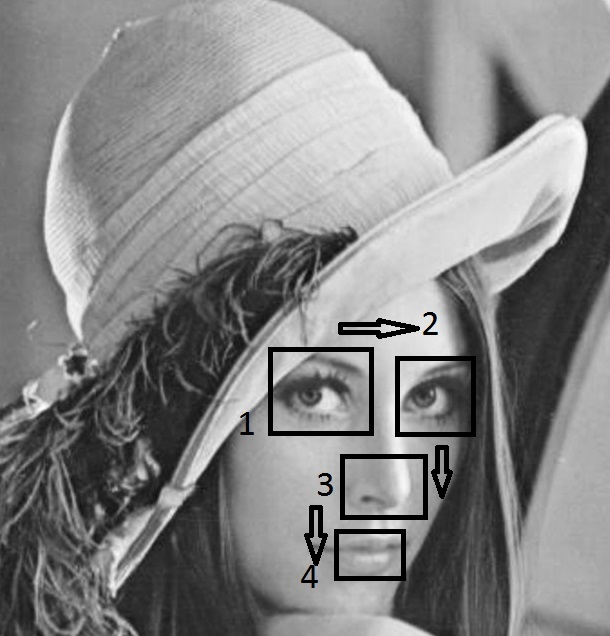
\includegraphics[width=0.5\textwidth]{misc/photos/face}
	\caption{Visual interpretation of the causal matrix. 1 --- detection area for the sensor responsible for the left eye, 2 for the right eye, 3 for the nose, and 4 for the mouth. The arrows indicate the time transitions (saccades) from the triggering one sensor to the next one.}		
\end{figure}

In the above example, each feature of the ``face'' sign image can also be represented by a sign in the actor’s world model. Thus, the case where the characteristic features of the sign image are sensor data is special. More generally, the sign image forming features are other signs corresponding to these characteristic features. Therefore, we can compare the image $p$ of the sign $s$ to the set $S_p(s)$ with the power $q$, each element of which corresponds to a causal matrix line number $z$ sized $q\times h$, i.e. each feature $s_i\in S_p(s)$ corresponds to a characteristic binary vector specifying discrete time moments of ones, during which this feature must be present in the input data in order to successfully recognize the sign $s$ image (to actualize the sign).

Each sign’s image can correspond to multiple causal matrices, setting various precedents of the presented object or process observation in the environment. All sequence of the sign $s$ image causal matrices will be denoted as $Z^p(s)$.

To clarify the definition of the set $S_p(s)$, we introduce a domain of embedded binary relationships $\{\sqsubset_p,\sqsubset_p^1,\sqsubset_p^2,\dots\}$ defined by the sign set $S$. We consider the sign $s_i$ as an \textit{element of the sign $s$ image} $(s_i,s)\in\sqsubset_p$ or $s_i\sqsubset_p s$ if $s_i\in S_p(s)$. If it is known that the sign $s_i$ is corresponded by one in the $t$-th column of the sign $s$ causal matrix $z\in Z^p(s)$, we will use the relationship $\sqsubset_p^t$ so that $\sqsubset_p^t\subset \sqsubset_p$.

\subsection{Sign image recognition }\label{subsec:actual}

Let us briefly describe the algorithm of sign image recognition (sign actualization) in Figure \ref{fig:percept}. We will consider the sign images to be grouped according to the set $S_p(s)$ similarity into nodes organized as hierarchical structures (for details, \cite{Osipov2015d}). Lower-level nodes include causal matrices of signs that are features for the signs, the causal matrices of which are included in higher-level nodes. These nodes and sign image causal matrices are formed as a result of education \cite{Skrynnik2016}; in this algorithm version, we consider all matrices and nodes to be formed and not updated. Further, we will restrict ourselves to the case where all matrices within one node have the same number of columns, which is a natural condition due to the matrix similarity. The period of time, during which all node causal matrix columns are processed, is called the computing cycle of the node.

\begin{figure}
	\centering
	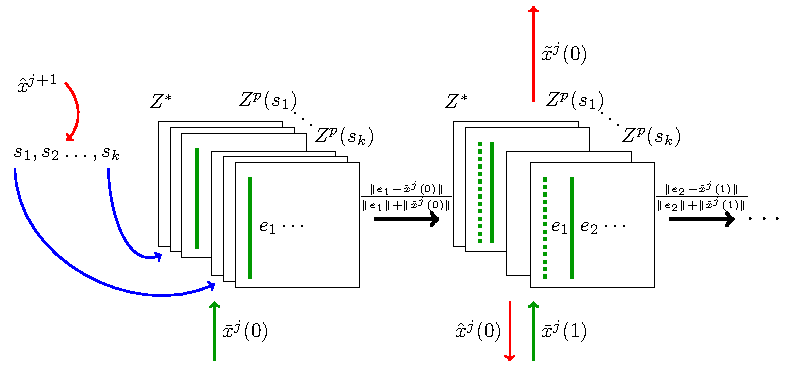
\includegraphics[width=0.8\textwidth]{algo/perception}
	\caption{Scheme of the sign image recognition algorithm.}
	\label{fig:percept}		
\end{figure}

The algorithm input data is certain initial time $\tau_s$, recognizable feature prediction vector at this hierarchy level $\hat x^{j+1}(\tau_s)$ and the input function $\omega^j$ setting the sequence of the event input vectors $\bar x(t)$. As a result of the algorithm, the output function $\vec \eta^j$ is formed, which is a sequence of recognizable feature vectors, and an expectation function, which is the vector sequence of a prediction event for the recognizable features of the  lower level hierarchy.

The recognition computing cycle in the level $j$ node starts with defining the initial node’s state through a real vector of the hierarchy upper level - the expectation vector $\hat x^{j+1}(\tau_s)$ formed on the basis of the upper level node status (steps \ref{alst:init_start}--\ref{alst:init_end} at the time moment $\tau_s$). The initial state is defined as a sign subset where the images are predicted on the basis of the expectation vector. We introduce a constant $c_1$ determining the threshold of the recognizable image predicted weight, above which the relevant causal matrices fall into the active matrix set $Z^*$ (step \ref{alst:select_f}). Next, causal matrices are selected from the set of active ones; for these, the usual distance $\|x\|=\sum_i |x_i|$ according to the first column rate $e_1$ from the event $\bar x^j(0)$ at the initial moment of time does not exceed the constant $c_2$ (step \ref{alst:select_z}). The updated set of active causal matrices obtained this way is the current state of the node (step \ref{alst:init_state}). On the basis of the active causal matrices, the output node vector is calculated by the voting method at the initial moment of time $\tilde x^j(0)$ (steps \ref{alst:init_calc_out2} -- \ref{alst:init_calc_out3}).

\linespread{1}
\begin{algorithm}[H]
	\label{alg:automato}
	\begin{algorithmic}[1]
				\Require $\tau_s, \hat x^{j+1}(\tau_s)$, $\omega^j$ - input function.
		\Ensure $\varphi^j$ - expectation function, $\vec\eta^j$ - output function.

		\State $F^*=\varnothing,Z^*=\varnothing,t=0$; 
		\State $c_1\in(0,1), c_2\in(0,1)$;

		\Statex \Comment{initialize the state}
				
		\ForAll{components $\hat x_k^{j+1}$ of the vector $\hat x^{j+1}(\tau_s)=(\hat x_1^{j+1},\hat x_2^{j+1},\dots,\hat x_l^{j+1})$} \label{alst:init_start}
			\If{$\hat x_k^{j+1}{\ge}c_1$} \label{alst:select_f}
				\State $F^*=F^*\cup\{s_k\}$;
			\EndIf
		\EndFor
		
		\State $\bar x(0):=\omega^j(\tau_s)$;
		
		\ForAll{signs $s_k\in F^*$}
			\ForAll{causal matrices $z\in Z^p(s_k)$}
				\If{$\frac{\|e_1-\bar x^j(0)\|}{\|e_1\|+\|x^j(0)\|}<c_2$} \label{alst:select_z}
					\State $Z^*:=Z^*\cup\{z\}$;
				\EndIf
			\EndFor
		\EndFor
		
		\State $Z^*$ - initial node state; \label{alst:init_state}
		\State $\bar N=(|\{z|z\in Z^*,z\in Z^p(s_1)\}|,\dots,|\{z|z\in Z^*,z\in Z^p(s_l)\}|)$; \label{alst:init_calc_out2}
		\State $\eta(0):=\tilde x^j=W(\bar N)$; \label{alst:init_calc_out3}
		\State $\varphi^j(0):=\hat x^j=W(\sum_{s_k\in F^*}\hat x_k^{j+1}\sum_{z\in Z^*}e_2(z))$;\label{alst:init_control}
		\label{alst:init_end}
		\algstore{algst:store1}
	\end{algorithmic}
\end{algorithm}
\linespread{2}

The expectation vector $\hat x^j(0)$ is determined as a normalized vector, the $s$-th component of which is equal to the sum of all $s$-th elements of the causal active matrix second columns with weights corresponding to the elements of the expectation vector $\hat x^{j+1}(\tau_s)$ (step \ref{alst:init_control}). Since the idea of the future input signal is used (the second column of the causal matrices), $\hat x^j(0)$ is the expectation vector for the lower level hierarchy.

\linespread{1}
\begin{algorithm}[H]
	\begin{algorithmic}[1]
		\algrestore{algst:store1}
			\Statex \Comment{main circle}
	
	\State $t=1$;
	\While{$t\leqslant{h^j}-1$} \label{alst:cycle_start}
		\State $\bar x^j:=\omega(t)$;
	
		\ForAll{causal matrices $z$ in the set $Z^*$}
			\If{$\frac{\|e_t-\bar x^j(t)\|}{\|e_t\|+\|\bar x^j\|}\geqslant{c_2}$} \label{alst:update_z}
				\State $Z^*=Z^*\setminus\{z\}$;
			\EndIf
		\EndFor
	
		\State $Z^*$ - current state; 
		
		\State $\bar N=(|\{z|z\in Z^*,z\in Z^p(s_1)\}|,\dots,|\{z|z\in Z^*,z\in Z^p(s_l)\}|)$; \label{alst:calc_out1}
		\State $\eta(t):=\tilde x^j=W(\bar N)$; \label{alst:calc_out3}
	
		\State $t=t+1$;
		\If{$t\leqslant h^j-2$}
			\State $\varphi^j(t):=\hat x^j=W(\sum_{s_k\in F^*}\hat x_k^{j+1}\sum_{z\in Z^*}\bar e_t(z))$; \label{alst:calc_state1}
		\EndIf
	\EndWhile \label{alst:cycle_end}
	
	\Return $\varphi^j,\vec\eta^j$.
	\end{algorithmic}
\end{algorithm}
\linespread{2}

After determining the initial state, the main cycle starts working, which repeats the output vector and state calculation at the following moment until the time exceeds the characteristic node time $h^j$ (the number of causal matrix columns, steps \ref{alst:cycle_start}--\ref{alst:cycle_end}). At the beginning of this stage, the state, i.e. the set of active causal matrices $Z^*$, is updated due to removal of the matrices, the corresponding columns of which are much different from the current event $\bar x^j(t)$ (step \ref{alst:update_z}). Next, the output vector $\tilde x^j(t)$ is calculated by the voting method, according to the matrix number in the set of active causal matrices corresponding to the image (steps \ref{alst:calc_out1}--\ref{alst:calc_out3}).

At the end of the main cycle, the expectation output vector is calculated for the next moment of time $\hat x^j(t)$. The expectation vector is equal to the normalized vector, the elements of which are equal to the column element sum of the active causal matrices corresponding to the current moment of time regarding the weights of the initial expectation vector $\hat x^{j+1}(\tau_s)$ (step \ref{alst:calc_state1}).

\subsection{Causal network}

We introduce a special procedure $\Lambda_p: 2^Z\rightarrow 2^{\mathbb N}\times 2^{\mathbb N}$, which associates two disjoint column index subsets $I^c\subset\mathbb N, \forall i\in I^c\ i\leq h$ and $I^e\subset\mathbb N, \forall i\in I^e\ i\leq h$ ($\Lambda_p(Z^p(s))=(I^c,I^e)$) with each sequence $Z^p(s)\subset Z$ of the sign $s$ image causal matrices, so that $I^c\cap I^e=\varnothing$. The set $I^c$ will be called condition column indices, and the set $I^e$ will be called effect column indices. For example, if the procedure $\Lambda_p$ provides two sets $\{1\}$ and $\{2\}$ for the matrix sequence $Z$ consisting of only one matrix $((1, 0), (0, 1))$, this means that the appearance of an feature corresponding to the first matrix row causes the appearance of an feature corresponding to the second matrix row in the sequence. Thus, the procedure $\Lambda_p$ establishes a causal relationship regarding the set of input events and can be implemented in various ways including FCO, Norris algorithms, etc. \cite{Kuznetsov2001,Kuznetsov1996}. In this paper, we will consider only the cases where the causal matrix columns belong to two subsets (conditions and effects). There may be situations when the causal matrix columns form a chain of causes and effects; in this case, the function $\Lambda_p$ will issue more than two column subsets.

If the effect column set for the sign  $s$ image matrices $Z^p(s)$ is not empty $I^e \not=\varnothing$, we assume that the sign is an action or process, the result of which is encoded in the effect columns and its condition is encoded in the condition columns (the corresponding sign is procedural). Otherwise, if the effect column set of the sign $s$ image matrices $Z^p(s)$ is empty  $I^e=\varnothing$, i.e. if it cannot be determined which events precede others by the causal matrix sequence, we will consider the causal relationship as not being established, and consider the sign to represent an object or situation (the corresponding sign is object).

The following statements are true concerning the properties of the procedure $\Lambda_p$:
\begin{itemize}
	\item $I^c\cap I^e=\varnothing$ --- the causal matrix column cannot be both the condition and the effect at the same time,
	\item $|I^c\cup I^e|=h$ --- other column types, except the condition and effect ones, are absent,
	\item $I^c\not = \varnothing$ --- among the causal matrix columns, there must be at least one condition column, whereas the effect one may be absent (in the case of object features),
	\item $\forall i\in I^e, j\in I^c\ i>j$ --- all conditions precede the effects in time.
\end{itemize}

\begin{figure}[H]
	\centering
	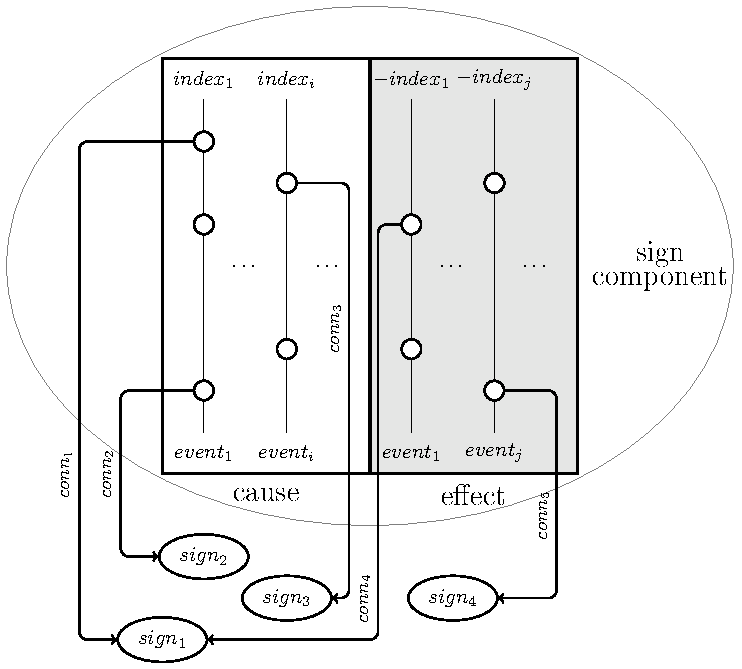
\includegraphics[width=0.6\textwidth]{causnet/caus_matr}
	\caption{Causal matrix example}	
	\label{fig:caus_matr}	
\end{figure}

Proceeding to the notation used at the semantic level of the model (section \ref{sec:semantic}), we can consider the causal matrix $z$ to be a rule $r=\langle F_C(z),F_A(z),F_D(z)\rangle$, in which
\begin{itemize}
	\item $F_C (z)\subseteq S_p(s)$ --- is a set of the features-conditions for the rule: $\forall f\in F_C(z)$ $f\sqsubset_p^i s, i\in I^c$;
	
	\item $F_A(z)\subseteq S_p(s)$ --- is a set of the features added by the rule: $\forall f\in F_A(z)$ $f\sqsubset_p^i s,i\in I^e, f\not\sqsubset^j f_p, j\in I^c$;
	
	\item $F_D(z)\subseteq S_p(s)$ --- is a set of the features deleted by the rule: $\forall f\in F_D(z)$ $f\not\sqsubset^i s, i\in I^e,f\sqsubset^j s, j\in I^c$.
\end{itemize}

The causal matrix example based on the above is shown in Figure \ref{fig:caus_matr}.

Now, we introduce the notion of causal network, which will determine the heterarchy of the causal matrix set. The causal network $W_p=\langle V_p, E_p \rangle$ is a labelled directed graph, in which
\begin{itemize}
	\item each node $v\in V_p$ corresponds to the sign $s$ image causal matrix sequence $Z^p(s)$, referred to as $v\rightarrow Z^p(s)$;
	\item the edge $e=(v_1, v_2)$ belongs to the graph edge set $E$ if $v_1\rightarrow Z^p(s_1), v_2\rightarrow Z^p(s_2)$ and $s_1\in S_p(s_2)$, i.e. if the sign $s_1$ is an element of the image $s_2$;
	\item each graph edge $e=(v_1, v_2), v_1\rightarrow Z^p(s_1), v_2\rightarrow Z^p(s_2)$ is associated with a label $\epsilon=(\epsilon_1,\epsilon_2,\epsilon_3)$ --- a sequence of three integers:
	\begin{itemize}
		\item $\epsilon_1$ - the index of the original matrix in the sequence $Z^p(s_1)$ can accept a special 0 value, if the sources are matrices of the sequence
		\item $\epsilon_2$ --- the index of the target matrix in the sequence $Z^p(s_2)$, the row of which is associated with the feature $s_1$;
		\item $\epsilon_3$ --- the column index in the target matrix, in which there is 1 in the row corresponding to the feature $s_1$, can accept positive (condition columns) and negative values (effect columns).
	\end{itemize}		
\end{itemize}

The causal network is a special type of non-uniform semantic network \cite{Osipov1990}. An example of such network is given in Figure \ref{fig:caus_net}.

\begin{figure}[h]
	\centering
	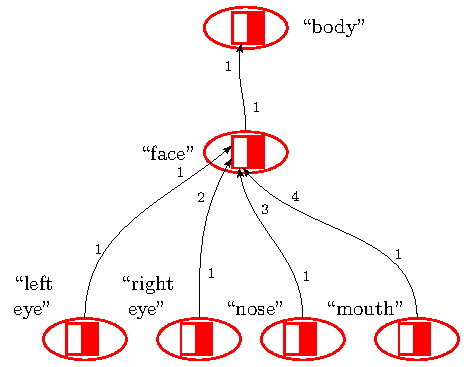
\includegraphics[width=0.5\textwidth,page=1]{examples/causnet/en/caus_net_colored_en}
	\caption{Causal network example of the sign image set. Here, the causal matrices are shown as squares; the condition columns are the left white parts of the squares, the effect columns are the right black parts of the squares. The $\epsilon_1$ label is displayed at the start of each arrow, the $\epsilon_2$ label is the square number, at which the arrow points, and the $\epsilon_3$ label is displayed at the end of each arrow.}
	\label{fig:caus_net}		
\end{figure}

Similarly, the causal networks are determined for the other sign components --- for significance and personal meaning. For each sign $s$, the sets$S_m(s)$ and $S_a(s)$ are determined, i.e. the domains of embedded relationships $\{\sqsubset_m,\sqsubset_m^1,\sqsubset_m^2,\dots\}$ are a \textit{significance element} and $\{\sqsubset_a,\sqsubset_a^1,\sqsubset_a^2,\dots\}$ are a \textit{meaning element}. The set $S_m(s)$ is interpreted as the role composition of the $s$ sign, i.e. subdomain elements or the action role in accordance with the semantic level of the model. The set $S_a(s)$ is interpreted as an instant component constitution of the situation observed and experienced by the actor holding world model or action committed by the actor at the moment. The sets $Z^m(s)$, $Z^a(s)$ and procedures $\Lambda_m$, $\Lambda_a$ are similarly determined.

Three types of causal networks differ from each other due to the relationships generated on the basis of these networks for the corresponding set of sign components, the operations performed in these networks, and the role the play during the implementation of cognitive functions such as behaviour planning \cite{Osipov2015d,Panov2017a}. Now, we can clarify the definition of the sign \cite{Osipov2015c} using the introduced formalism of the causal matrices and causal networks.

\begin{definition}
	As the sign, we consider $s=\langle n, p, m, a \rangle$, where $n$ is the sign name, $p=Z^p$ is the sign image, i.e. the causal matrix sequence corresponding to a certain causal network node with images regarding all input and output links, $m=Z^m$ is the sign significance, i.e. the causal matrix sequence corresponding to a certain causal network node with significances regarding all input and output links, and $a=Z^a$ is the sign image, i.e. the causal matrix sequence corresponding to a certain causal network node with personal meanings regarding all input and output links.
\end{definition}

Further, we will assume that each sign has a significance, i.e. $Z^m\not = \varnothing$. If the sign has no image, i.e. $Z^p=\varnothing,S_p=\varnothing$, it will be called the \textit{category sign} (we will distinguish between metaconcepts and categories). Finally, if the sign has no assigned personal meaning, i.e. $Z^a=\varnothing, S_a=\varnothing$, it will be called \textit{impersonal}.

\section{Semiotic network}\label{sec:semnetwork}

Next, we determine three domains of sign set binary relationships generated on the basis of the fragment structure of the three causal network types, including the respective sign components. These relationships correspond to the relationships introduced at the semantic level.

\subsection{Relationships on the set of images}	

Let us start with determining the sign set relationship generated with causal network images. This requires determining equality, similarity, inclusion and opposition for two causal matrices:

\begin{definition}
	Two causal matrices $z_1$ and $z_2$ are equal ($z_1=z_2$) if and only if the matrix dimensions are equal, sets of effect and condition column coincide $\Lambda({z_1})=\Lambda({z_2})$, and each binary vector $e_t^1$, matrix column $z_1$ are equal to corresponding binary vector $e_t^2$, and matrix column $z_2$.
\end{definition}

\begin{definition}
	Two causal matrices $z_1$ and $z_2$ are similar ($z_1\sim z_2$) if and only if there are two binary vectors $e_i$ and $e_j$, matrix columns $z_1$ and $z_2$, and their by-component multiplication (i.e. multiplication of the components corresponding to the same feature; if the corresponding feature is absent in the vector, it is believed that there is zero in its place) is not equal to the zero vector $e_i*e_j\not = 0$, and both of them are either condition columns $i\in I^c(z_1), j\in I^c(z_2)$ or effect columns $i\in I^e(z_1), j\in I^e(z_2)$.
\end{definition}

\begin{definition}
	The causal matrix $z_1$ is included in the causal matrix $z_2$ ($z_1\subseteq z_2$) if and only if any binary vector $e_i$, matrix column $z_1$ have a binary vector $e_j$, matrix column $z_2$, so that $e_i | e_j=e_j$ ($|$ is bit-by-bit ``or''), and both of them are either condition columns $i\in I^c(z_1), j\in I^c(z_2)$ or effect columns $i\in I^e(z_1), j\in I^e(z_2)$.
\end{definition}

\begin{definition}
	Two causal matrices  $z_1$ and $z_2$ are opposed to each other ($z_1\perp z_2$) if and only if the dimensions of the matrices are equal, the sets of effect and condition column indices coincide $\Lambda({z_1})=\Lambda({z_2})$ and each binary vector $e_t^1$, matrix $z_1$ column have no intersection with the respective binary vector $e_t^2$, matrix $z_2$ column, i.e. $e_t^1\& e_t^2=0$, where $\&$ is bit-by-bit ``and''.
\end{definition}

In addition to the previously introduced relationship domain ``be an image element'' ${\sqsubset_p, \sqsubset_p^1, \dots}$, based on the relationship definitions for the set of causal matrices, we determine four relationships based on the sign set $S$.

\begin{definition}
	The pair of signs $s_1$ and $s_2$ belong to \textit{the image equivalence relationship} $R_{eq}^p$, $(s_1,s_2)\in R_{eq}^p$, if the sequence $Z^p(s_1)=\langle z_1^1,z_2^1,\dots\rangle$ is point-wise equal to the sequence $Z^p(s_2)=\langle z_1^2,z_2^2,\dots\rangle$, i.e. their power is equal and every causal matrix of the first sequence is equal to the corresponding matrix of the second sequence, i.e. $|Z^p(s_1)| = |Z^p(s_2)|, \forall z_t^1\in Z^p(s_1)\ \exists z_l^2\in Z^p(s_2): z_t^1=z_l^2, t=l$.
\end{definition}

\begin{definition}\label{def:sim}
	The pair of signs $s_1$ and $s_2$ belong to \textbf{the image similarity relationship} $R_{sim}^p$, $(s_1,s_2)\in R_{sim}^p$, if each causal matrix $z_i$ in the sequence $Z^p(s_1)$ has a similar matrix $z_j$ in the sequence $Z^p(s_2)$, i.e. $\forall z_i\in Z^p(s_1)\ \exists z_j\in Z^p(s_2): z_i\sim z_2$.
\end{definition}

\begin{definition}
	The pair of signs $s_1$ and $s_2$ belong to \textbf{the image inclusion relationship} $R_{in}^p$, $(s_1,s_2)\in R_{in}^p$, if each causal matrix $z_i$ in the sequence $Z^p(s_1)$ has an inclusive matrix $z_j$ in the sequence $Z^p(s_2)$, i.e. $\forall z_i\in Z^p(s_1)\ \exists z_j\in Z^p(s_2): z_i\subseteq z_2$.
\end{definition}

\begin{definition}
	The pair of signs $s_1$ and $s_2$ belong to \textbf{the image opposition relationship} $R_{con}^p$, $(s_1,s_2)\in R_{con}^p$, if the power of the sequence $Z^p(s_1)=\langle z_1^1,z_2^1,\dots\rangle$ is equal to the power of the sequence $Z^p(s_2)=\langle z_1^2,z_2^2,\dots\rangle$, and each causal matrix of the first sequence is opposed to the corresponding matrix of the second sequence, i.e. $|Z^p(s_1)| = |Z^p(s_2)|, \forall z_t^1\in Z^p(s_1)\ \exists z_t^2\in Z^p(s_2): z_t^1\perp z_t^2$.
\end{definition}

Regarding the definitions introduced, the image relationship domain $R^p$ is formed by the relationships of ``being an image element'', image equivalence, similarity, inclusion and opposition.

\subsection{Relationships on the set of significances}	

The domain of significance relationships $R^m$ includes the relationships ``being a significance element'' ${\sqsubset_m,\sqsubset_m^1,\dots}$ and, similarly to the image case, relationships of significance equivalence $R_{eq}^m$, similarity $R_{sim}^m$, inclusion $R_{in}^m$ and opposition $R_{con}^m$.

In addition, an important role in the significance network during the cognitive function modelling is played by the following two relationships: the classification relationship $R_{cl}^m$, causal relationship $R_{cas}^m$ and scenario relationship $R_{sc}^m$.

\begin{figure}[H]
	\centering
	\includegraphics[width=0.6\textwidth,page=2]{examples/causnet/en/caus_net_colored_en}
	\caption{Example of relationship elements in the significance causal network. Here, the set $\{(s_2,s_3),(s_2,s_4),(s_2,s_5),(s_2,s_6),(s_1,s_2)\}\subset R_{cl}^m$ is interpreted as ``square, triangle, circle and trapezoid are geometric shapes that are objects for drawing action''. The set $\{(s_7,s_1),(s_7,s_8),(s_7,s_9)\}\subset R_{sc}^m$ is interpreted as ``the drawing action is determined by the roles of the actor (the person who is drawing), the tool (used to make the drawing), and the object (what is drawn)''. The symbols are the same as in Figure \ref{fig:caus_net}.}
	\label{fig:signif_relat}		
\end{figure}

\begin{definition}
	The pair of signs $s_1$ and $s_2$ belong to \textbf{the relationship of classification} $R_{cl}^m$ if $s_1$ is the category object sign and there is only one sign $s_1$ significance causal matrix with a single column, in which the only one corresponds to the sign $s_2$, i.e. $Z^p(s_1)=\varnothing, I^e(s_1)=\varnothing, \exists z\in Z^m(s_1): h(z)=1, |e_1(z)|=1, s_2\sqsubset_m^1 s_1$.
\end{definition}

\begin{definition}
	The pair of signs $s_1$ and $s_2$ belong to \textbf{the scenario relationship} $R_{sc}^m$, $(s_1,s_2)\in R_{sc}^m$ if $s_1$ is the procedural sign, $s_2$ is the object sign, possibly, the category sign, and the sign $s_2$ is the sign $s_1$ significance element, i.e. $I^e(s_1)\not = \varnothing, I^e(s_2) = \varnothing, s_2\sqsubset_m s_1$.
\end{definition}

Examples of relationship elements $R_{cl}^m$ and $R_{sc}^m$ are shown in Figure \ref{fig:signif_relat}.

\subsection{Relationships on the set of personal meanings}	
The domain of personal meaning relationships $R^a$ includes the relationships ``be a meaning element'' ${\sqsubset_a,\sqsubset_a^1,\dots}$ and, similarly to the image case, relationships of meaning equivalence $R_{eq}^a$, similarity $R_{sim}^a$, inclusion $R_{in}^a$ and opposition $R_{con}^a$.

Also, we introduce situational relationships of the personal meaning set $R_{sit}^a$.

\begin{definition}
	The pair of signs $s_1$ and $s_2$ belong to \textbf{the situational relationship} $R_{sit}^a$, $(s_1,s_2)\in R_{sit}^a$, if $s_1$ is the procedural sign, $s_2$ is the object sign not included in the category, and the sign $s_2$ is the sign $s_1$ meaning element, i.e. $I^e(s_1)\not = \varnothing, I^e(s_2) = \varnothing, S_p(s_2)=\varnothing, s_2\sqsubset_a s_1$.
\end{definition}

On the basis of the situational relationship's definition, it is possible to introduce the concept of situation determined on the basis of a procedural sign with all the object signs not included in the categories, together with which it constitutes a situational relationship.

\begin{definition}
	The sign set $Sit=\{s_1,s_2,\dots,s_n\}$ will be called the \textbf{situation} if $s_1$ is the only procedural sign in the $Sit$ set and for all $1<i\leq n\ s_i\in Sit, (s_1,s_i)\in R_{sit}^a$.
\end{definition}

Example of the relationship elements $R_{sit}^a$ and situation is provided in Figure \ref{fig:mean_relat}.

\begin{figure}[h]
	\centering
	\includegraphics[width=0.7\textwidth,page=3]{examples/causnet/en/caus_net_colored_en}
	\caption{Example of the relationship $R_{sit}^a$ elements in the meaning causal network. Here, the set $\{(s_5,s_1),(s_5,s_2),(s_5,s_3),(s_5,s_4)\}\subset R_{sit}^a$ is equivalent to the situation ``Ivan draws a trapezoid with a pencil''. The symbols are the same as in Figure \ref{fig:caus_net}.}
	\label{fig:mean_relat}		
\end{figure}

\subsection{Semiotic network}
\textit{The semiotic network} consists of five elements $\Omega=\langle W_p, W_m, W_a, R, \Theta \rangle$, where
\begin{itemize}
	\item $W_p, W_m, W_a$ --- are causal networks of the image, significance and personal meaning sets respectively,
	\item $R$ --- is the domain of sign set relationships formed on the basis of three causal networks, i.e.  $R=\{R^p, R^m, R^a\}$,
	\item $\Theta$ --- is the domain of sign set operations (which are defined below).
\end{itemize} 


\section{The structure of operations in the semiotic network }\label{sec:operations}
At the structural level of the world model simulation, we clarify the definitions of operations functioning in the world model and those generating new signs or scenarios on the basis of two input sign components. In other words, the generation of, for example, a new image on the basis of two other sign images results in the formation of other new signs' components, according to the rules of the operation. In this paper, for each causal network, the definitions will be given as examples using the ones given at the semantic level in the section \ref{sec:semantic}. For the sake of simplicity, we will consider each sign component as being characterized by one causal matrix (one action, one rule). Further, the procedure of the new sign formation described in \cite{Osipov2014c} will be used and denoted here as $\Psi$.

\subsection{Operation of generalization}
Generalization is a key cognitive process enabling the organization of knowledge in a hierarchical form, and the creation of compact representations of objects and processes within reality. In psychology, there are three kinds of generalization: syncrete, complex and concept \cite{Vygotsky1999}. During a syncretic generalization, the leading role is played by sign's personal meaning, i.e. the subjective attitude of the actor's world model to the represented objects. During the formation of complex generalization, the sign images and objectively existing features are used. Concept generalization is based on sign significances and it is formed in the process of reviewing generic-specific relationships, the knowledge of which is coordinated with other participants of the common activity.

Let us define the operation of \textbf{image generalization} (complex generalization formation) as $\Theta^p: S\times S\rightarrow S$. Let $s_1=\langle n_1, \{z_1^p\}, \{z_1^m\}, \{z_1^a\} \rangle$, $s_2=\langle n_2, \{z_2^p\}, \{z_2^m\}, \{z_2^a\} \rangle$ be signs, so that $(s_1,s_2)\in R_{eq}^p$, i.e. this exhibits similar relationships. The newly formed sign will be denoted as $s_3$.

According to the definition $\autoref{def:sim}$, this means that $z_1^p\sim z_2^p$, i.e. the causal matrices are similar. We define the new causal matrix $z_3^p$ as follows: $z_3^p=(e_1^3,e_2^3,\dots,e_h^3)$, where each column $e_i^3$ has a pair $e_j^1, e_k^2$ of matrix $z_1^p$ and $z_2^p$ respectively, so that $e_i^3=e_j^1*e_k^2\not=\varnothing$ and $i\in I^c(z_3^p), j\in I^c(z_1^p), k\in I^c(z_2^p)$. In other words, the matrix $z_3^p$ is a generalization of the matrices $z_1^p$ and $z_2^p$ containing only the events, which are an event generalization for both matrices.

Let $Z'_1$ and $Z'_2$ be sets of procedural causal matrices, for which the signs $s_1$ and $s_2$, accordingly, are features. In these two sets, we find a pair of similar causal matrices: $(z_1^m,z_2^m)$. Next, we define the procedural causal matrix $z_4^m$ --- a new matrix in the significance causal network, which entails the generalization of matrices $z_1^m$ and $z_2^m$: $z_4^m=(e_1^4,e_2^4,\dots)$, where each column $e_i^4$ has a pair of matrices $z_1^m$ and $z_2^m$ columns $e_j^1, e_k^2$, so that
\begin{itemize}
	\item -	in each of them, the reference to the corresponding sign significances $s_1$ and $s_2$ is replaced by a reference to the only empty matrix $z_3^m$ of the newly formed sign $s_3$,
	\item $e_i^4=e_j^1*e_k^2\not=\varnothing$ and 
	\item either simultaneously $i\in I^c(z_4^m), j\in I^c(z_1^m), k\in I^c(z_2^m)$, 
	\item or simultaneously  $i\in I^e(z_4^m), j\in I^e(z_1^m), k\in I^c(z_2^m)$.
\end{itemize}

According to the generated pair of matrices $z_3^p$ and $z_3^m$, we obtain a new sign $s_3$ with the help of the new sign generation procedure $\Psi$ as the operation $\Theta^p$ result; its image is a generalization of sign images $s_1$ and $s_2$, and its significance is a certain role in the generalized action with the signs$s_1$ and $s_2$. The newly formed procedural matrix $z_4^m$ can be included in a node of the existing significance network or serve as a separate node for a new sign, representing a new generalized action.

Here is an example of the image generalization operation. Let us have two signs $s_1$ and $s_2$ with the names \textit{``apple''} and \textit{``mandarin''} respectively. The causal matrices for the sign image components $s_1$ and $s_2$ are as follows (features are shown instead of ones):
\[
z_1^p = \begin{bmatrix}
0&0& \text{``green''} \\
0& \text{``round''} &0 \\
\text{``peel''} &0 &0  \\
\text{``thin''} &0 &0
\end{bmatrix}
z_2^p = \begin{bmatrix}
0&0& \text{``orange''} \\
0& \text{``round''} &0 \\
\text{``peel''} &0 &0  \\
\text{``thick''} &0 &0
\end{bmatrix}
\]
The sign significance components $s_1$ and $s_2$ are connected by the causal network to the procedural signs $s_3$ ``to peel an apple'' and $s_4$ ``to peel a mandarin'' (here, the vertical bar separates the condition and effect columns):
\[
z_3^m= \left[\begin{array}{ccc|cccc}
0&0&0&0&\text{``table''}&0\\
0&\text{``apple''}&0& 0&0&\text{``apple''}\\
0&0& \text{``knife''} &0 &0\\
0& 0& 0 &\text{``on''} &0&0\\
\text{``closely''}& 0& 0 &0 &0&0\\
\text{``peel''} &0 &0 &\text{``peel''}  &0&0\\
\text{``thin''} &0 &0 & \text{``thin''} &0&0
\end{array}
\right]
\]
\[
z_4^m= \left[\begin{array}{ccc|cccc}
0&0&0&0&\text{``table''}&0\\
0&\text{``mandarin''}&0& 0&0&\text{``mandarin''}\\
0&0& \text{``fingers''} &0 &0&0\\
0& 0& 0 &\text{``on''} &0&0\\
\text{``closely''}& 0& 0 &0 &0&0\\
\text{``peel''} &0 &0 &\text{``peel''}  &0&0\\
\text{``thick''} &0 &0 & \text{``thick''} &0&0
\end{array}
\right]
\] 
As a result of completing the  operation for generalizing the image $\Theta^p$, two signs are formed: generalization on the basis of the features of the sign's image $s_5$ named ``fruit'' and generalized on the basis of significance sign feature $s_6$ ``to peel'', which is a generalized action that can be done to the fruit:
\[
z_5^p = \begin{bmatrix}
0& \text{``round''} \\
\text{``peel''} &0
\end{bmatrix}
\]
\[
z_6^m= \left[\begin{array}{ccc|cccc}
0&0&0&0&\text{``table''}&0\\
0&\text{``fruit''}&0& 0&0&\text{``fruit''}\\
0& 0& 0 &\text{``on''} &0&0\\
\text{``closely''}& 0& 0 &0 &0&0\\
\text{``peel''} &0 &0 &\text{``peel''}  &0&0\\
\end{array}
\right]
\] 

\subsection{Closure operation by significances}
Another important cognitive function is the ability to generate possible scenarios based on the sign significances. This process plays a special role in the everyday world model, where most cognitive processes forming human behaviour, such as planning and communication, are based on finding, applying and forming new scenarios \cite{Osipov2015d}. In the simplest case, the scenario means an action, in which the particular role performers are fixed, i.e. the scenario is a specified action. Formally, the scenario is the sign set $Scen=\{s_1,s_2,\dots, s_n\}$, where the only procedural sign is $s_1$, and all other signs form two subgroups: $S_r$ is the set of role signs and $S_o$ is the set of scenario participant signs. The role signs of the set $S_r$ are category signs associated with the $s_1$ scenario relationship $R_{sc}^m$. The participant signs of the set $S_o$ are either not the signs not being the category signs associated with the $s_1$ scenario relationship $R_{sc}^m$ or signs belonging to the classification relationship $R_{cl}^m$ being paired with other signs of the set $S_r$.

We define \textit{the closure operation by significances} $\Theta^m$, which forms the scenario $Scen$ according to some procedural sign $s$: $\Theta^m(s)=Scen$. In fact, the scenario formation means the iterative inclusion of the signs in the set $Scen$ when considering the relationship elements $R_{cl}^m$ and $R_{sc}^m$:

\begin{itemize}
	\item [Step 1] Include the procedural sign $s$ in the scenario $Scen=\{s\}$.
	\item [Step 2] Add the scenario with the signs associated with $s_1$ the scenario relationship: $Scen=Scen\cup\{s_i|(s_1,s_i)\in R_{sc}^m, I^e(s_i)=\varnothing\}$.
	\item [Step 3] Add the scenario with signs that are not category signs and that are associated with the scenario object signs by the classification relationship: $Scen=Scen\cup\{s_j|(s_i,s_j)\in R_{cl}^m, s_i\in Scen, I^e(s_i)=\varnothing, S_p(s_i)=\varnothing, S_p(s_j)\not=\varnothing\}$.
	\item [Step 4] Repeat the Step 3 until the scenario is no longer added with new signs or until all the signs of the set determined by the task have been tried. For example, during goal-setting, only a certain subset of the signs is used, which are candidates to the scenario formed \cite{Osipov2014c}.
\end{itemize}

An example of the generated scenario is shown in Figure \ref{fig:scenarion}.

\begin{figure}[h]
	\centering
	\includegraphics[width=\textwidth,page=4]{examples/causnet/en/caus_net_colored_en}
	\caption{Scenario example. The central procedural sign is $s_5$. The role signs are $S_r=\{s_1,s_2,s_3,s_4\}$, the participant signs are $S_o=\{s_7,s_8,s_9,s_{10},s_{11}\}$. The scenario relationship elements are marked by solid arrows, the classification relationships – by the broken ones. The rest of the symbols are the same as in Figure \ref{fig:caus_net}.}
	\label{fig:scenarion}		
\end{figure}


\subsection{Operation of meaning agglutination}
In conclusion, we present a typical example of the personal meaning network operation --- agglutination. The agglutination, fusion, of two sign meanings allows for the creation of a new meaning of the third sign, usually already present in the world model. In psychology, the new meaning is a combination of amalgamating data in experience elements, one of the main mechanisms for imagination and creative activities \cite{Asmolov1990}. Examples of the fusion of meanings include the allegorical figures by Leonardo da Vinci in the art and words like ``Moidodyr'' or ``Aibolit'' in linguistics.

Using the introduced formalism, we define the operation of agglutination: $\Theta^a$: $S\times S\rightarrow S$. Let $s_1=\langle n_1, \{z_1^p\}, \{z_1^m\}, \{z_1^a\} \rangle$, $s_2=\langle n_2, \{z_2^p\}, \{z_2^m\}, \{z_2^a\} \rangle$. The sign of the world model, which is being formed or already exists, is denoted by $s_3$. As a result of the operation $\Theta^a$, the sign $s_3$ receives a new meaning, represented by causal matrix $z_3^a$ which is built as follows. Let $z_1^a=(e_1^1, e_2^1,\dots,e_h^1)$ and $z_2^a=(e_1^2, e_2^2,\dots,e_l^2)$, the causal matrix is $z_3^a=(e_1^3, e_2^3,\dots,e_q^3)$, where $q=h+l$, $I^c(z_3^a)=I^c(z_1^a)\cup \{i+|I^c(z_1^a)||i\in I^c(z_2^a)\}$, $I^e(z_3^a)=I^e(z_1^a)\cup \{i+|I^e(z_1^a)||i\in I^e(z_2^a)\}$,
\[
e_t^3=\begin{cases}
e_t^1, &\text{if}\ t<|I^c(z_1^a)|,\\
e_{t-|I^c(z_1^a)|}^2, &\text{if}\ |I^c(z_1^a)|<t<|I^c(z_1^a)|+|I^c(z_2^a)|,\\
e_{t-|I^c(z_2^a)|}^1, &\text{if}\ |I^c(z_1^a)|+|I^c(z_2^a)|<t<|I^c(z_1^a)|+|I^c(z_2^a)|+|I^e(z_1^a)|,\\
e_{t-|I^c(z_1^a)|-|I^e(z_1^a)|}^2, &\text{if}\ t>|I^c(z_1^a)|+|I^c(z_2^a)|+|I^e(z_1^a)|.
\end{cases}
\]
Proceeding to the rule notation, we can say that the new meaning presented by the rule $z_3^a$ is the condition and effect unity of the rules $z_1^a$ and $z_2^a$: $F_C(z_3^a)=F_C(z_1^a)\cup F_C(z_2^a)$ and either $F_A(z_3^a)=F_A(z_1^a)\cup F_A(z_2^a)$, or $F_D(z_3^a)=F_D(z_1^a)\cup F_D(z_2^a)$ \cite{Osipov2016a}.

As an example, let us take the formation of a new personal meaning for the ``Saint Petersburg'' sign as a result of operations that  agglutinate (fuse) meanings of the ``newspaper'' and ``coffee'' signs, represented as the following matrices (actions ``read newspaper'', ``drink coffee''):

\[
z_1^a= \left[\begin{array}{ccc|cccc}
0&0&0&0&0&0&\text{``news''}\\
0&\text{``cafe''}&0&0&\text{``cafe''}&0&0\\
0&\text{``on''}&0&0 &\text{``on''}&0&0\\
0& 0& \text{``Nevsky''}&0 &0&\text{``Nevsky''}&0\\
\text{``newspaper''}&0&0&\text{``newspaper''}&0&0&0\\
\text{``in''} &0 &0 &\text{``in''}&0&0&0\\
0&0 &0 & 0 &0&0&0
\end{array}
\right]
\]
\[
z_2^a= \left[\begin{array}{ccc|cccc}
0&0&0&0&0&0&\text{``coffee''}\\
0&\text{``cafe''}&0&0&\text{``cafe''}&0&0\\
0&\text{``on''}&0&0 &\text{``on''}&0&0\\
0& 0& \text{``Nevsky''}&0 &0&\text{``Nevsky''}&0\\
\text{``cap''}&0&0&\text{``newspaper''}&0&0&0\\
\text{``in''} &0 &0 &\text{``in''}&0&0&0\\
0&0 &0 & 0 &0&0&0
\end{array}
\right]
\] 
The new causal matrix $z_3^a$ will be as follows. The condition columns represent the consistent unity of the matrix condition columns $z_1^a$ and $z_2^a$ (excess zero lines are omitted)
\[
\left[\begin{array}{cccccc}
0&\text{``cafe''}&0&0&\text{``cafe''}&0\\
0&\text{``on''}&0&0 &\text{``on''}&0\\
0& 0& \text{``Nevsky''}&0 &0&\text{``Nevsky''}\\
\text{``newspaper''}&0&0&0&0&0\\
0&0&0&\text{``cap''}&0&0\\
\text{``in''} &0 &0 &\text{``in''}&0&0
\end{array}
\right]
\]
The effect columns represent the consistent unity of the matrix effect columns $z_1^a$ and $z_2^a$ (excess zero lines are omitted)
\[
\left[\begin{array}{cccccccc}
0&0 &0 &\text{``news''}&0&0&0&0\\
0&0 &0 &0&0&0&0&\text{``coffee''}\\	
0&\text{``cafe''}&0&0&0&\text{``cafe''}&0&0\\
0&\text{``on''}&0&0&0 &\text{``on''}&0&0\\
0& 0& \text{``Nevsky''}&0&0 &0&\text{``Nevsky''}&0\\
\text{``newspaper''}&0&0&0&0&0&0&0\\
0&0&0&0&\text{``cap''}&0&0&0\\
\text{``in''} &0 &0&0&\text{``in''}&0&0&0
\end{array}
\right]
\]

In this case, we do not consider the matter of choosing the sign $s_3$, the new meaning of which is formed.

\section*{Conclusion}
This paper presents a new approach to the integration of the activity actor’s knowledge of the environment and its own features and also consideration of operations based on this knowledge --- the sign based world model. The world model simulation is described at the syntactic, semantic and structural levels. The four-component sign concept, which has been introduced in previous authors’ papers on the basis of neurophysiological and psychological considerations, is used. A special mathematical structure is introduced - the causal matrix integrating the static information representation in the form of the feature set and the procedural information as a rule with effects and conditions. Three types of semantic networks are introduced on the basis of the causal matrix set --- for image, significance and personal meaning causal networks. Using the presented formalism, it is possible to construct algorithms restoring relationships with the sign set modelling basic object links and processes of the external world. The paper describes important operations in the world model simulating of key cognitive functions of generalization, scenario formation and meaning agglutination.

\section*{Acknowledgment}
This work was supported by the Russian Foundation for Basic Research (Project No. 16-37-60055).

\section*{References}

\bibliography{swm_operations}

\end{document}